% !TEX root = main.tex

\newgeometry{top=2.170cm,
            bottom=3.510cm,
            inner=2.1835cm,
            outer=2.1835cm,
            ignoremp}

%% Title page

\begin{titlepage}
   \begin{center}
       \vspace*{4cm}

       \textbf{\Huge Improved microfading device for risk assessment of colour change in Van Gogh's works}
           
       \vspace{7cm}
       
       \textbf{\Large Gauthier Patin}          
              
   \end{center}
\end{titlepage}


%% Copyright page

\null%
\label{thesis:colophon}
\vfill
\pdfbookmark[1]{Colophon}{thesis:colophon}

Written in 2018--2023 by Gauthier Patin 

ISBN: 978909037535

Copyright \copyright \hspace{0.1cm}2023 by Gauthier Patin

Printed by Proefschriftmaken, \url{https://www.proefschriftmaken.nl}\\

\vspace{0.5cm}

\textbf{Colophon} \\

This thesis was typeset with the help of \LaTeX{} and to a large extent uses the source code provided by Ken Arroyo Ohori for his PhD thesis (\url{https://github.com/kenohori/thesis}). Most of the figures were created using Matplotlib package inside Jupyter notebooks, or Inkscape.

The source code of this thesis is available at: \url{https://github.com/g-patin/PhD_thesis}

A digital version of this dissertation is available on the Digital Academic Repository of the University of Amsterdam (\url{https://dare.uva.nl}) as well on my PhD website (\url{https://microfadingphd.wordpress.com}). 

The data that have been used to create the figures in Chapters 3, 4, and 5 have been stored on a Zenodo repository (\url{https://zenodo.org/record/8216110}). \\

\vspace{0.5cm}

\textbf{Cover} \\

The front and back covers are based on the results of light ageing experiments conducted during this PhD using the methodology described in Chapter 4 (section \ref{sec:DL_methodology}) of this dissertation. Both covers display the results of daylight exposure on an eosin paint-out (PO098). The front cover shows visualization of colour patches as the light dose increases from 0 to 120 MJ/m\textsuperscript{2}, while the back cover shows differences in the reflectance spectra as the light dose increases from 0 to 120 MJ/m\textsuperscript{2}. A value of 120 MJ/m\textsuperscript{2} roughly corresponds to 50 years of continuous exposure in the galleries of the Van Gogh Museum (10 hours per day at 50 lux).



%% A two-page pdf provided to me by the UvA once my dissertation had been accepted.

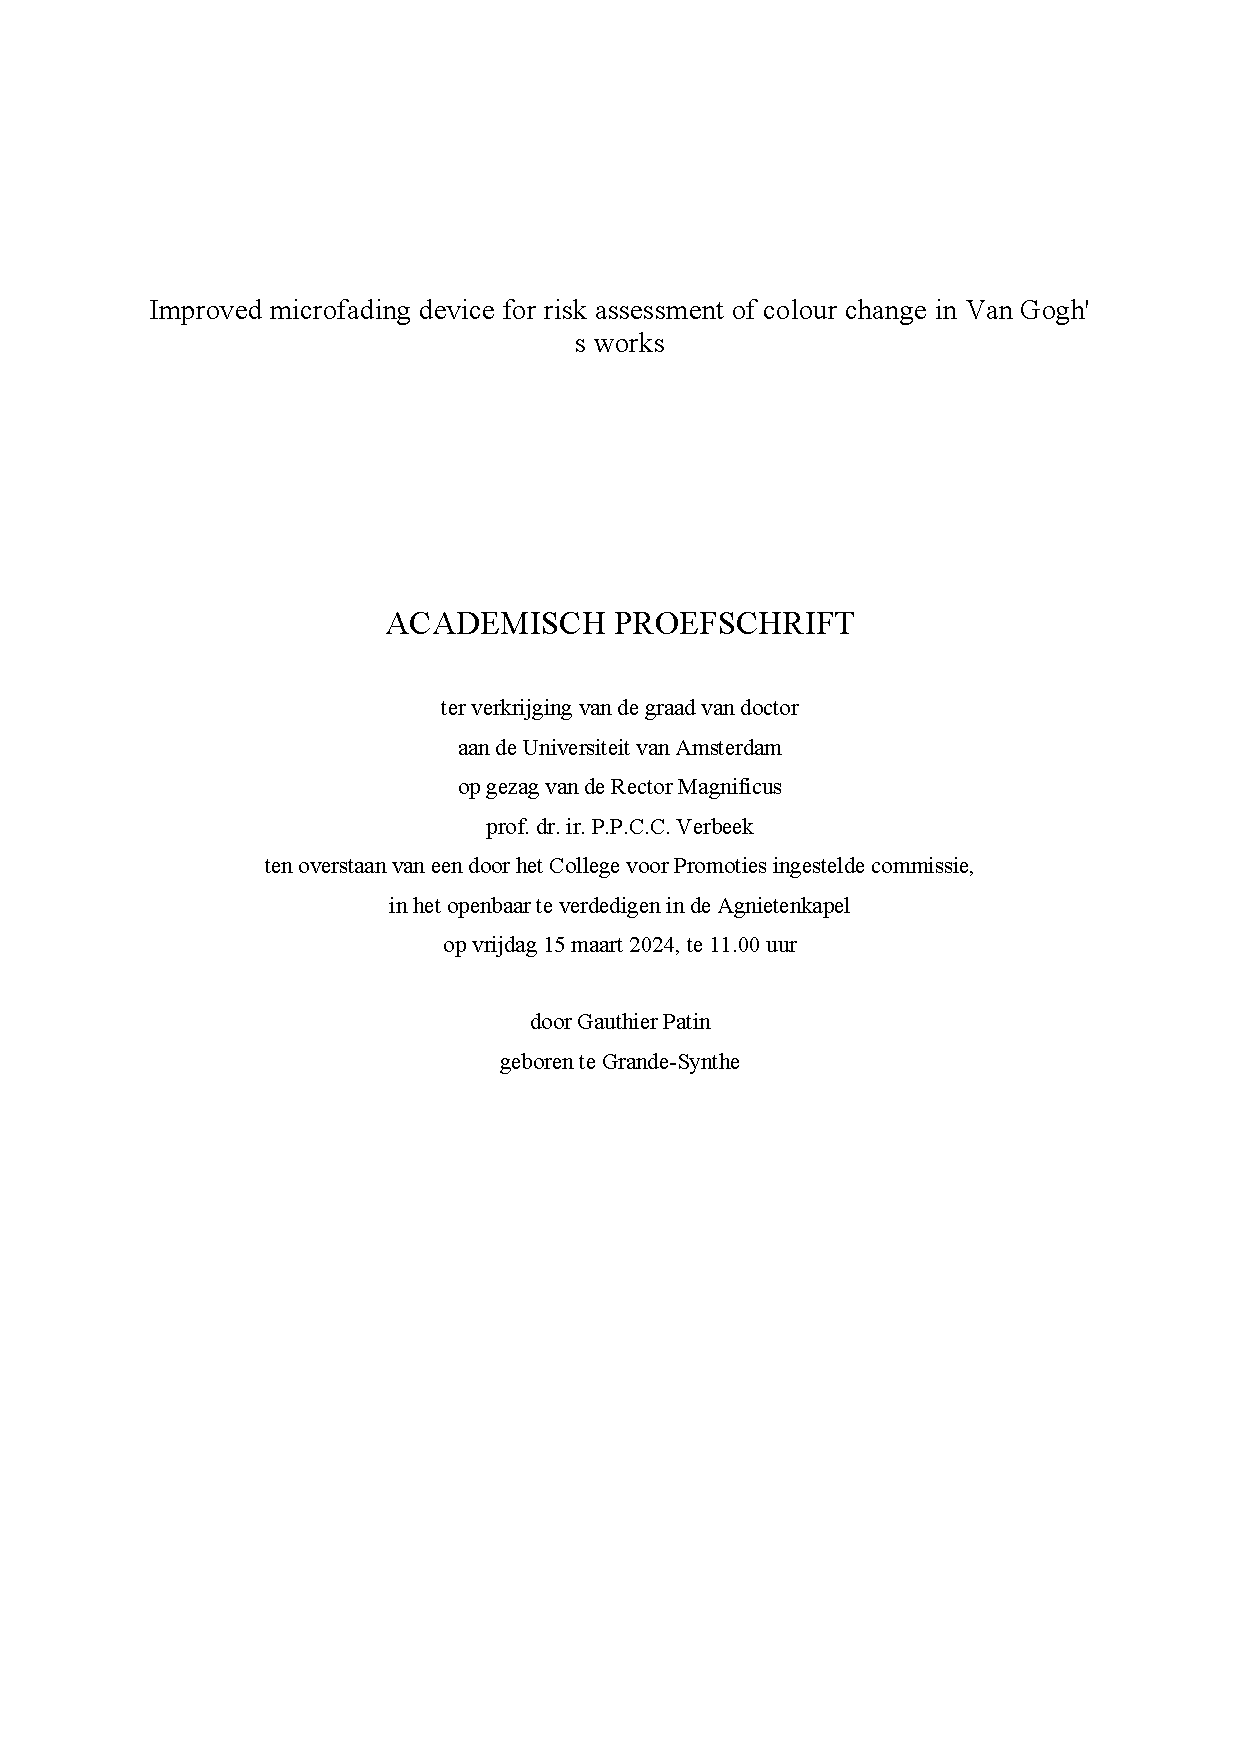
\includepdf[pages=1]{P30_ATTACH.pdf}
\includepdf[pages=2]{P30_ATTACH.pdf}


%% Funding statement

\newpage
{\Large\textbf{Funding}}\\

The research for this thesis received financial assitance from the AXA Research Fund, the Van Gogh Museum-ASML Partnership in Science, the Rijksdienst voor het Cultureel Erfgoed, and the Rijksmuseum Amsterdam. 

\vspace{1.5cm}

\begin{figure}[!h]
\centering

\includegraphics[width=0.75\textwidth]{Logo_institutions.png}
\label{fig:colours_description}
\end{figure}

\newpage
